\documentclass[titlepage]{article}
\usepackage[utf8]{inputenc}

\title{
  \textbf{Dokumentacja} \\
  System do zarządzania boiskiem szkolnym}
\date{January 2021}

\author{Develop Team}
\usepackage{natbib}
\usepackage[T1]{fontenc}
\usepackage{graphicx}
\usepackage{polski}
\usepackage{indentfirst}
\usepackage{sectsty}
\usepackage{hyperref}
\usepackage{listings}




\begin{document}

\maketitle
\tableofcontents
\section*{Wstęp}
\addcontentsline{toc}{section}{Wstęp}

Głównym założeniem tej aplikacji jest rezerwowane boiska za pomocą strony internetowej. Zapewnia nam ona logowanie poprzez CAS. Cały projekt składa się z 
\begin{itemize}
  \item Aplikacji Bacekndowej opatej o Node.js
  \item Aplikacji frontendowej opartej o React.js
  \item Aplikacji frontendowej (administrator) opartej o ReactAdmin.js
\end{itemize}

Aplikacja korzysta z architektury REST oraz jest dostosowana do urządzeń mobilnych

\newpage
\section{Backend}

\begin{figure}[h]
\centering
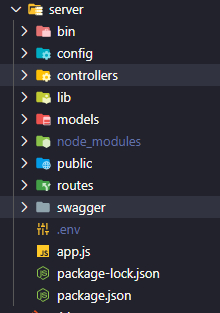
\includegraphics[width=0.5\textwidth]{struktura.png}
\caption{Struktura backendu}
\label{fig:obrazek struktura}
\end{figure}

\indent Część backendu w aplikacji do zarządzania boiskiem szkolnym jest napisany w języku JavaScript oparta o framework Express.js.


\subsection{Katalog config}
W tym katalogu mieszczą się dwa pliki
\begin{figure}[h]
\centering
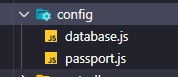
\includegraphics[width=0.5\textwidth]{config.png}
\caption{config katalog}
\label{fig:obrazek config}
\end{figure}
\subsubsection{database.js}
Ustawiamy z której bazy danych chcemy korzystać. Ustala się to zmienną NODE\_ENV w pliku .env
\subsubsection{passport.js}
Zawierają się tam wszystkie ustawienia od autoryzacji użytkownika (CAS oraz logowanie niezależne)

\subsection{Katalog controllers}
Katalog zawiera pliki które zawierają funkcje służące do działania całej aplikacji, są one eksportowane i podpinane pod ścieżki w folderze routes

\begin{figure}[h]
\centering
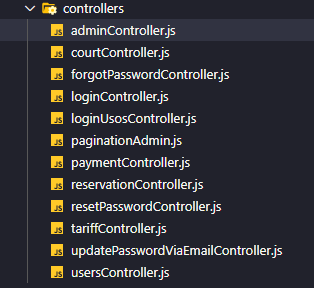
\includegraphics[width=0.5\textwidth]{controllers.png}
\caption{controllers katalog}
\label{fig:obrazek controllers}
\end{figure}

\subsubsection{adminController.js}
Plik ten zawiera wszystkie funkcje, potrzebne to zarządzania aplikacją frontedową przez administratora systemu. 

\subsubsection{courtController.js}
Tworzymy tutaj rozkład boiska który chcemy aby był dostępny dla naszych klientów

\subsubsection{forgotPasswordController.js}
Funkcje odpowiedzialne za przypominanie hasła

\subsubsection{loginController.js}
Logowanie i wylogowywanie użytkownika z aplikacji (outh)

\subsubsection{loginUsosController.js}
Logowanie i wylogowywanie użytkownika z aplikacji (CAS) \\
Link do dokuemntacji: \url{https://apps.usos.edu.pl/developers/api/}

\subsubsection{paginationAdmin.js}
Middleware do aplikacji adminstratora pomagające ustalić podział rekordów na strony

\subsubsection{paymentController.js}
Metody odpowiedzialne za wytworzenie tokenu w serwisie Pay'u oraz dokonanie płatności

\subsubsection{reservationController.js}
Controller odpowiedzialny za tworzenie rezerwacji, modyfikacji, usuwania.

\subsubsection{resetPasswordController.js}
Sprawdzenie czy możemy ustawić nowe hasło

\subsubsection{tariffController.js}
Dodawanie, modyfikowanie i usuwanie cennika obiektu

\subsubsection{updatePasswordViaEmailController.js}
Controller do wygenerowania nowego hasła

\subsubsection{usersController.js}
Tworzymy nowego użytkownika oraz modyfikujemy jego dane personalne

\newpage
\subsection{Katalog lib}
Katalog z bibliotekami

\begin{figure}[h]
\centering
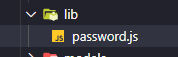
\includegraphics[width=0.5\textwidth]{lib.png}
\caption{lib katalog}
\label{fig:obrazek lib}
\end{figure}

\subsubsection{password.js}
Generujemy hash z hasła oraz sprawdzamy czy hasło jest poprawne 

\subsection{Katalog models}
Katalog z modelami bazy danych

\begin{figure}[h]
\centering
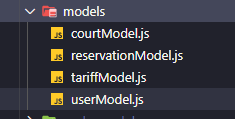
\includegraphics[width=0.5\textwidth]{models.png}
\caption{models katalog}
\label{fig:obrazek models}
\end{figure}

\subsubsection{courtModel.js}

\begin{lstlisting}[
  language={JavaScript},
  caption={courtModel}
]const mongoose = require('mongoose');

const courtModel = mongoose.Schema({
  ids: {
    type: String,
    required: true,
  },
  nameCourt: {
    type: String,
    required: true,
  },
  description: {
    type: String,
    required: true,
  },
  date: [
    {
      nameOfDay: String,
      value: Boolean,
    },
  ],
});
module.exports = mongoose.model('courtModel', courtModel);


\end{lstlisting}

Model Court składa się z:
\begin{itemize}
  \item ids (id)
  \item nameCourt (nazwa obiektu)
  \item description (część boiska)
  \item date (data w którym dniu boisko jest dostępne)
\end{itemize}


\subsubsection{reservationModel.js}

\begin{lstlisting}[
  language={JavaScript},
  caption={courtModel}
]
const { ObjectID, ObjectId } = require('mongodb');
const mongoose = require('mongoose');

const reservationModel = mongoose.Schema({
  start_time: {
    type: String,
    required: true,
  },
  hour: {
    type: String,
    required: true,
  },
  courtId: {
    type: String,
    required: true,
  },
  userId: {
    type: ObjectId,
    ref: 'userModel',
    required: true,
  },
});
module.exports = mongoose.model('reservationModel', reservationModel);



\end{lstlisting}

Model Reservation składa się z:
\begin{itemize}
  \item start\_time (kiedy rezerwacja zaczyna się)
  \item hour (ile godzin trwa)
  \item courtId (id boiska)
  \item userId (id usera)
\end{itemize}

\subsubsection{tariffModel.js}

\begin{lstlisting}[
  language={JavaScript},
  caption={courtModel}
]
const mongoose = require('mongoose');

const courtsTariff = mongoose.Schema({
  ids: {
    type: String,
    required: true,
  },
  name: {
    type: String,
    required: true,
  },
  classes_and_sports_training: {
    type: String,
    required: true,
  },
  tournament_matches: {
    type: String,
    required: true,
  },
  university_club: {
    type: String,
    required: true,
  },
});
module.exports = mongoose.model('courtsTariff', courtsTariff);

\end{lstlisting}

Model tariff składa się z:
\begin{itemize}
  \item ids (id)
  \item name (nazwa obiektu)
  \item classes\_and\_sports\_training (jeden z typów cennika)
  \item tournament\_matches (jeden z typów cennika)
  \item university\_club (jeden z typów cennika)
\end{itemize}


\subsubsection{userModel.js}

\begin{lstlisting}[
  language={JavaScript},
  caption={courtModel}
]
const mongoose = require('mongoose');

const userModel = mongoose.Schema({
  email: String,
  hash: String,
  salt: String,
  idUsos: String, //usos
  student_status: String, //usos
  student_number: String, //usos
  name: String,
  surname: String,
  age: Number,
  phone_number: String,
  sex: String,
  role: {
    type: String,
    default: 'user',
  },
  adress_street: String,
  adress_city: String,
  adress_postalCode: String,
  isStudent: {
    type: Boolean,
    default: false,
  }, //usos
  isActive: {
    type: Boolean,
    default: true,
  },
  nip: String,
  resetPasswordToken: String,
  resetPasswordExpires: Date,
});

module.exports = mongoose.model('userModel', userModel);

\end{lstlisting}

Model user składa się z:
\begin{itemize}
  \item email (email użytkownika)
  \item hash (hash hasła)
  \item salt (sól do hasła)
  \item idUsos (id użytkownika podczas logowania poprzez CAS)
  \item student\_status (czy jest studentem aktywnym)
  \item name (imie użytkownika)
  \item surname (nazwisko użytkownika)
  \item age (wiek użytkownika)
  \item phone\_number (numer telefonu użytkownika)
  \item sex (płeć użytkownika)
  \item role (admin czy użytkownik)
  \item adress\_street (miejsce zamieszkania użytkownika - ulica)
  \item adress\_city (miejsce zamieszkania użytkownika - miasto)
  \item adress\_postalCode (miejsce zamieszkania użytkownika - kod pocztowy)
  \item isStudent (czy zalogowany poprzez CAS)
  \item isActive (czy użytkownika ma nadal aktywne konto)
  \item nip (NIP użytkownika)
  \item resetPasswordToken (token do resetowania hasła)
  \item resetPasswordExpires (czas w którym możemy zresetować hasło)
  
\end{itemize}

\newpage
\subsection{Katalog routes}
Katalog z modelami bazy danych

\begin{figure}[h]
\centering
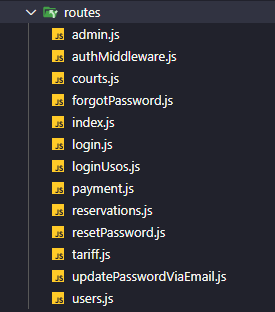
\includegraphics[width=0.5\textwidth]{routes.png}
\caption{routes katalog}
\label{fig:obrazek routes}
\end{figure}

\subsubsection{admin.js}

\begin{tabular}{l12}

\hline
\textbf{Metoda} & \textbf{Endpoint} & \textbf{Opis}\\
\hline
GET & /api/admin & Spradzanie czy zalogowany jako admin\\
\hline
GET & /api/admin/users & Zwraca wszystkich użytkowników\\
\hline
GET & /api/admin/users/:userId & Zwraca usera o podanym ID\\
\hline
GET & /api/admin/reservations & Zwraca usera o podanym ID\\
\hline
DELETE & /api/admin/reservations/:id & Usuwa rezerwajce o podanym ID\\
\hline
POST & /api/admin/reservations & Tworzenie rezerwacji przez administratora\\
\hline
\end{tabular}


\subsubsection{authMiddleware.js}
Middleware potrzebne do sprawdzania role użytkownika, oraz do wyświetlania danych w panelu administratora

\subsubsection{courts.js}
\begin{tabular}{l12}

\hline
\textbf{Metoda} & \textbf{Endpoint} & \textbf{Opis}\\
\hline
GET & /api/admin/courts & Zwraca podział boiska dla administratora\\
\hline
GET & /api/courts & Zwraca podział boiska\\
\hline
POST & /api/admin/courts & Tworzenie boiska w panelu administratora\\
\hline
DELETE & /api/admin/courts/:courtId & Usuwanie boiska o danym ID\\
\hline
PATCH & /api/admin/courts/:courtId & Aktualizacja boiska\\
\hline
GET & /api/admin/courts/:courtId & Zwraca boisko/strefę o podanym ID\\
\hline
\end{tabular}

\subsubsection{forgotPassword.js}
\begin{tabular}{l12}

\hline
\textbf{Metoda} & \textbf{Endpoint} & \textbf{Opis}\\
\hline
POST & /api/forgotPassword & Zapomniane hasło\\
\hline

\end{tabular}

\subsubsection{login.js}
\begin{tabular}{l12}

\hline
\textbf{Metoda} & \textbf{Endpoint} & \textbf{Opis}\\
\hline
POST & /api/login/ & Logowanie do panelu administratora\\
\hline
POST & /api/login/:role & Logowanie do aplikacji\\
\hline
GET & /api/logout & Wylogowanie\\
\hline

\end{tabular}

\subsubsection{loginUsos.js}
\begin{tabular}{l12}

\hline
\textbf{Metoda} & \textbf{Endpoint} & \textbf{Opis}\\
\hline
GET & /api/loginUsos & Logowanie przez CAS\\
\hline
GET & /api/loginUsos/connect & Logowanie przez CAS\\
\hline
GET & /api/loginUsos/callback & Callback przy logowaniu przez CAS\\
\hline
GET & /api/loginUsos/logout & Wylogowanie użytkownika przy logowaniu przez CAS\\
\hline

\end{tabular}

\subsubsection{payment.js}
\begin{tabular}{l12}

\hline
\textbf{Metoda} & \textbf{Endpoint} & \textbf{Opis}\\
\hline
POST & /api/getToken & Generowanie tokenu do płatności\\
\hline
POST & /api/createPayment & Tworzenie płatności\\
\hline
POST & /notify & Powiadomienia o sukcesie czy porażce przy dokonowaniu płatności\\
\hline
GET & /getPaymentInfo/:orderId & Infromacje o zamówieniu o podanym ID\\
\hline

\end{tabular}

\subsubsection{reservations.js}
\begin{tabular}{l12}

\hline
\textbf{Metoda} & \textbf{Endpoint} & \textbf{Opis}\\
\hline
GET & /api/reservations & Zwraca wszystkie rezerwacje\\
\hline
POST & /api/reservations/getPrice & Cena dla danej rezerwacji\\
\hline
GET & /api/allReservations & Wszystkie rezerwacje\\
\hline
POST & /api/reservation/create & Tworzenie rezerwacji\\
\hline
POST & /api/reservation/create/groups & Tworzenie grupowych rezerwacji\\
\hline
DELETE & /api/reservation/delete/:reservationId & Usuwanie rezerwacji o podanym ID\\
\hline
PATCH & /api/reservation/update/:reservationId & Aktualizacja rezerwacji o podanym ID\\
\hline
GET & /api/reservation/:reservationId & Zwraca rezerwacje o podanym ID\\
\hline
GET & /api/reservations/:userId & Rezerwacje danego użytkownika\\
\hline

\end{tabular}

\subsubsection{resetPassword.js}
\begin{tabular}{l12}

\hline
\textbf{Metoda} & \textbf{Endpoint} & \textbf{Opis}\\
\hline
GET & /api/reset & Resetowanie hasła\\
\hline

\end{tabular}

\subsubsection{tariff.js}
\begin{tabular}{l12}

\hline
\textbf{Metoda} & \textbf{Endpoint} & \textbf{Opis}\\
\hline
GET & /api/admin/priceLists & Zwraca podział cen na wszystkie obiekty\\
\hline
GET & /api/admin/priceLists/:id &  Cena o podanym ID\\
\hline
PUT & /api/admin/priceLists/:id &  Update cennika\\
\hline
GET & /api/priceLists &  Zwraca podział cen na wszystkie obiekty dla aplikacji frontendowej\\
\hline

\end{tabular}

\subsubsection{updatePasswordViaEmail.js}
\begin{tabular}{l12}

\hline
\textbf{Metoda} & \textbf{Endpoint} & \textbf{Opis}\\
\hline
PATCH & /api/updatePasswordViaEmail & Ustawia nowe hasło\\
\hline

\end{tabular}

\subsubsection{user.js}
\begin{tabular}{l12}

\hline
\textbf{Metoda} & \textbf{Endpoint} & \textbf{Opis}\\
\hline
GET & /api/checkAuthUser & Sprawdzamy czy użytkownik ma autoryzację\\
\hline
POST & /api/user/create & Tworzenie nowego użytkownika\\
\hline
PATCH & /api/user/update & Aktualizacja danych użytkownika\\
\hline
GET & /api/user/:userId & Zwraca użytkownika o podanym ID\\
\hline

\end{tabular}

\newpage
\subsection{Katalog swagger}
Katalog z plikami do tworzenia dokumentacji online projektu

\begin{figure}[h]
\centering
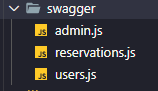
\includegraphics[width=0.5\textwidth]{swagger.png}
\caption{swagger katalog}
\label{fig:obrazek swagger}
\end{figure}

\subsection{Plik .env}
W tym pliku umieszczamy potrzebne zmienne, klucze, ustawienia których nie chcemy udostępniać w kodzie. Plik musi być utworzony przed pierwszym uruchomieniem projektu.

\begin{lstlisting}[
  language={JavaScript},
  caption={courtModel}
]
DB_CONNECTION = ''
DB_CONNECTION_PROD = ''
DB_CONNECTION_ATLAS = ''
DB_CONNECTION_ATLAS_TEST = ''
NODE_ENV = ''
USOS_CONSUMER_KEY = ''
USOS_CONSUMER_SECRET = ''
OAUTH_SECRET = ''
ROLE_ADMIN = ''
ROLE_USER = ''
EMAIL_ADDRESS = ''
EMAIL_PASSWORD = ''
PAYU_CLIENT_ID = ''
PAYU_CLIENT_SECRET = ''

\end{lstlisting}

\subsection{Plik app.js}
Główny plik projektu w którym umieszczamy niezbędne konfiguracje



\end{document}
